\documentclass[11pt, letterpaper]{report}
\input{../../../../report.tex}
\title{General Physics 2: Lab 3 Report}
\date{11/02/24}
\renewcommand{\thesection}{\arabic{section}}
\pagestyle{plain}
\pgfplotsset{width=10cm}
\begin{document}
\maketitle
\begin{abstract}
	This paper identifies the charge to mass ratio of the election $e /m_e$, which is already known to be approximately $(1.7588047\pm 0.0000049)\cdot 10^{11}\,\text{C}/\text{kg}$. Using two different methods, we find values of $e /m_e = 2.03\cdot 10^{11}$ and $e /m_e = 2.15\cdot 10^{11}$, which do not agree with the accepted value within our error bounds. We conclude our experiment had many sources of error, possibly including the experimental apparatus itself.
\end{abstract}
\section{Introduction}
A particle with charge $q$ and velocity $\mathbf{v}$ moving in a uniform magnetic field $\mathbf{B}$ experiences the Lorentz force
\begin{equation}\label{eq:1}
	\mathbf{F}=q \mathbf{v}\times \mathbf{B}
.\end{equation}
For this paper, it's more convenient to exclusively consider the magnitudes of the given vectors. We will thus make use of the representation
\begin{equation}\label{eq:2}
	F=qvB\sin \theta 
,\end{equation}
where $\theta $ is the angle formed between $\mathbf{v}$ and $\mathbf{B}$. From this, it's obvious that $v$ will remain constant, since $\mathbf{F}$ always acts perpendicular to $\mathbf{v}$.

To minimize the amount of measurements we must take and error we must account for, we will design our experimental apparatus such that $\theta =90^\circ $. We then have
\begin{equation}\label{eq:3}
	F=qvB
.\end{equation}
Additionally, we know the charged particle will take a circular path within the magnetic field, so we can use Newton's second law for circular motion, which states
\begin{equation}\label{eq:4}
	\Sigma F=\frac{mv^2}{R}
.\end{equation}
We can design our experimental apparatus such that $\mathbf{v}$ is rather large, and thus we claim the effects of gravity will be negligable. Since electrons are small, we also claim air resistance is negligable. Thus, the Lorentz force is the only force the electrons experience, and we have
\begin{equation}\label{eq:5}
	qvB=\frac{mv^2}{R}
.\end{equation}
Since we want to measure the charge to mass ratio of an electron, we want to solve for $q / m$. Rearranging and simplifying, we have
\begin{equation}\label{eq:6}
	\frac{q}{m}=\frac{v}{BR}
.\end{equation}
Therefore, provided we know the magnetic field $B$ of our experimental apparatus and the velocity $v$ of the electrons, we can measure the radius $R$ to identify the value of $e /m_e$.
\section{Procedures}
We use a cathode ray tube (CRT) to generate an electron beam, which are accelerated to a velocity $v$ by a potential difference $V$ inside the tube. Since $qV=K=\frac{1}{2}mv^2$, we know $eV=\frac{1}{2}m_ev^2$, and thus
\begin{equation}\label{eq:7}
	v^2 = \frac{2eV}{m_e}
.\end{equation}
By varying $V$, we are thus able to vary $v$ by a factor proportional to $\sqrt{V} $.

We will generate a magnetic field using two Helmholtz coils of diameter $d$, placed at a distance $d / 2$ apart. Given this setup, the strength of the magnetic field is proportional to the magnitude of the current flowing through the coils
 \begin{equation}\label{eq:8}
	 B=\left( 4.23\cdot 10^{-3} \right) I
.\end{equation}
Although this equation is only precise at the center of the experimental apparatus, we claim it is a sufficient approximation for the magnetic field the electron experiences, so long as the electrons remain approximately centered between the coils. Using this relation, we can find $B$ given a value of $I$. Moreover, we can vary  $I$ to vary $B$ linearly, allowing us to make more measurements.

Finally, we will use a piece of photoluminescent paper with grid markings on it to make precise measurements of the displacement of the electron beam in both the horizontal and vertical directions. If we claim the electrons start at the point $(0,0)$ and curve through the point $(x,y)$, then we can identify the radius $R$ of the circle they travel on by forming a triangle and applying the pythagorean theorem.
\begin{center}
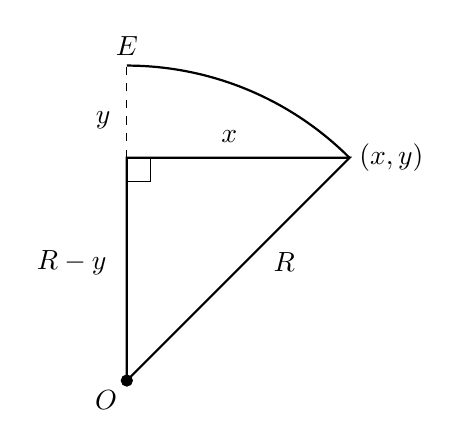
\begin{tikzpicture}
	% Define the center and radius
  \coordinate (O) at (0,0); % Center of the circle
  \def\radius{4} % Radius of the arc

  % Define points for the arc and triangle
  \coordinate (A) at (0,\radius); % Starting point of the arc (top center)
  \coordinate (B) at ({\radius*cos(45)}, {\radius*sin(45)}); % End point of the arc, 45 degrees to the right
  \coordinate (C) at (0,{\radius*sin(45)});

  % Draw the circular arc from A to B
  \draw[thick] (A) arc[start angle=90, end angle=45, radius=\radius cm];
  
  % Draw the right triangle
  \draw[thick] (O) -- (C) -- (B) -- cycle;
  \draw[dashed] (C) -- (A);

  % Draw and label the center
  \filldraw (O) circle (2pt) node[below left] {$O$};

  % Label points A and B
  \node[above] at (A) {$E$};
  \node[right] at (B) {$(x,y)$};
  \node at (-0.7,1.5) {$R-y$};
  \node at (2,1.5) {$R$};
  \node at (-0.3,3.3) {$y$};
  \node at (1.3,3.1) {$x$};

  % Mark the right angle at C
  \draw (0,{\radius*sin(45)-0.3}) -- (0.3,{\radius*sin(45)-0.3}) -- (0.3,{\radius*sin(45)});
\end{tikzpicture}\\
\noindent Figure 1: Identifying $R$ from $(x,y)$ Coordinate\label{fig:1}
\end{center}
Using figure \ref{fig:1}, we know from the pythagorean theorem that $R^2=x^2+\left( R-y \right) ^2$, and thus
\begin{equation}\label{eq:9}
	R=\frac{x^2}{2y}+\frac{y}{2}
.\end{equation}

We now have a method of controlling the magnetic field $B$, controlling the electron's velocity $v$, and identifying the resultant radius $R$ from any given conditions. However, there may be extraneous magnetic fields, such as the Earth's magnetic field, that also act on the electrons. We can call this error $B_\varepsilon$. If this field is assumed to be constant, then if it forms an angle $\phi $ with $\mathbf{v}$, by equation \ref{eq:2} we will have
\[
	F_{+}=qv(B+B_{\varepsilon }\sin \phi )
.\]
If we switch the direction of our magnetic field, then we must add a factor of $180^\circ $ to $\phi $ in order to keep our original $B$ positive inside the cross product. Notice that $\sin \left( \phi +180 \right) =-\sin \phi $. We then have
\[
	F_{-}=qv(B-B_{\varepsilon }\sin \phi )
.\]
Notice that
\[
	F_{+}+F_{-}=qvB+qvB_{\varepsilon }\sin \phi +qvB-qvB_{\varepsilon }\sin \phi =2qvB=2F
.\]
Therefore, we can switch the direction of the magnetic field $\mathbf{B}$ and then average the results to minimize the error induced by extraneous fields.

In addition to this, we will perform many measurements at varying $I$ and $V$ values, which induce varying $B$ and $v$ values, which can be calculated later. With these understandings, we can propose the following procedures. These procedures constitute two different methods of measureing the information, one in which we fix a coordinate, and one in which we fix a potential. Both should give similar results.
\begin{enumerate}
	\item Fix some $(x,y)$ coordinate, and choose a few varying values of $V$. For each value, adjust the value of $I$ such that the electron beam passes through $(x,y)$. Record all values.
	\item Reverse the current, and repeat step 1 for the coordinate $(x,-y)$. Record all values.
	\item Now fix some potential difference $V$, and choose various points $(x,y)$. Adjust $I$ such that the electron beam passes through each $(x,y)$. Record all values.
	\item Reverse the current, and repeat step 3 for each coordinate $(x,-y)$.
\end{enumerate}
\section{Analysis}
\subsection{Data Record}
We chose the $(x,y)$ value $(10,2)$ for steps 1 and 2 of the procedure. The error in our current measurements was $\pm 0.0005$A for each measurement, and the error in our potential measurements was $\pm 1$V for each measurement. These error values hold for both table \ref{tab:1} and \ref{tab:2}, and will be considered more indepth in section \ref{sec:3.3}. For steps 3 and 4, we chose $V=3$V, and measured current at a few points.
\begin{center}
	Table 1: Experiment Results for $(x,y)=(10,2)$\label{tab:1}\vspace{5pt}\\
	\begin{tabular}{rrr}
		\toprule
		Potential (V)&Current (A)&Reversed Current (A)\\
		\midrule
		2000&0.129&0.127\\
		2300&0.139&0.135\\
		2600&0.149&0.142\\
		2900&0.156&0.151\\
		3200&0.162&0.159\\
		\bottomrule
	\end{tabular}\vspace{10pt}\\
	\noindent Table 2: Experimental Results for $V=3$V\label{tab:2}\vspace{5pt}\\
	\begin{tabular}{rrrr}
		\toprule
		Current (A)&Reversed Current (A)&$x$ (m)&$y$ (m)\\
		\midrule
		0.083&0.075&0.1&0.01\\
		0.102&0.094&0,09&0.01\\
		0.126&0.118&0.08&0.01\\
		0.165&0.152&0.07&0.01\\
		0.215&0.198&0.06&0.01\\
		\bottomrule
	\end{tabular}
\end{center}
\subsection{Data Analysis}
In accordance with our previous discussion, we averaged the current and reverse current from tables \ref{tab:1} and \ref{tab:2} before proceeding with other calculations. We then calculated the magnetic field $B$ using equation \ref{eq:8} For example, when the potential was $2000$, we had an average current of $0.128$, and thus a magnetic field of
\[
	B=\left( 4.23\cdot 10^{-3} \right) 0.128=0.000541
.\]
We then calculated $R$ using equation \ref{eq:9}, and got
\[
	R=\frac{x^2}{2y}+\frac{y}{2}=\frac{0.01}{0.04}+0.01=0.26
.\]
Finally, we absorbed equations \ref{eq:7} and \ref{eq:8} into \ref{eq:6} to obtain
\begin{equation}\label{eq:10}
	\frac{e}{m_e}=\frac{2V}{B^2R^2}
.\end{equation}
We can use this equation to calculate $e /m_e$. For example, when $V=2000$, we have
\[
	\frac{e}{m_e}=\frac{4000}{0.000541^2\cdot 0.26^2}=2.02\cdot 10^{11}
.\]
Using these equations, we produced table \ref{tab:1}.
\begin{center}
	Table 3: Calculated Values for $(x,y)=(10,2)$\label{tab:3}\vspace{5pt}\\
	\begin{tabular}{rrrr}
		\toprule
		Potential (V)&Average Current (A)&Magnetic Field (T)&$e /m_e$ (C/kg)\\
		\midrule
		2000&0.128&0.000541&$2.02\cdot 10^{11}$\\
		2300&0.137&0.000580&$2.03\cdot 10^{11}$\\
		2600&0.146&0.000615&$2.03\cdot 10^{11}$\\
		2900&0.154&0.000649&$2.04\cdot 10^{11}$ \\
		3200&0.161&0.000679&$2.05\cdot 10^{11}$ \\
		\bottomrule
	\end{tabular}
\end{center}
Our average value for $e /m_e$ using this method is then
\[
	\frac{e}{m_e}=2.03\cdot 10^{11}\; \text{C/kg}
.\]

Table \ref{tab:4} used all of the same calculations, but used table \ref{tab:2} as the initial set of data, rather than table \ref{tab:1}.
\begin{center}
	Table 4: Calculated Values for $V=3$V\label{tab:4}\vspace{5pt}\\
	\begin{tabular}{rrrr}
		\toprule
		Average Current (A)&Radius (m)&Magnetic Field (T)&$e /m_e$ (C/kg)\\
		\midrule
				   0.079&0.505&0.000334&$2.11\cdot 10^{11}$\\
				   0.098&0.410&0.000415&$2.08\cdot 10^{11}$\\
				   0.122&0.325&0.000516&$2.13\cdot 10^{11}$ \\
		     0.159&0.250&0.000670&$2.14\cdot 10^{11}$ \\
		     0.207&0.185&0.000873&$2.30\cdot 10^{11}$ \\
		\bottomrule
	\end{tabular}
\end{center}
Using this method, our average value for $e /m_e$ is thus
\[
	\frac{e}{m_e}=2.15\cdot 10^{11}
.\]

An interesting thing we can do with the results of the second experiment is plot $B$ vs $1 /R$.
\begin{center}
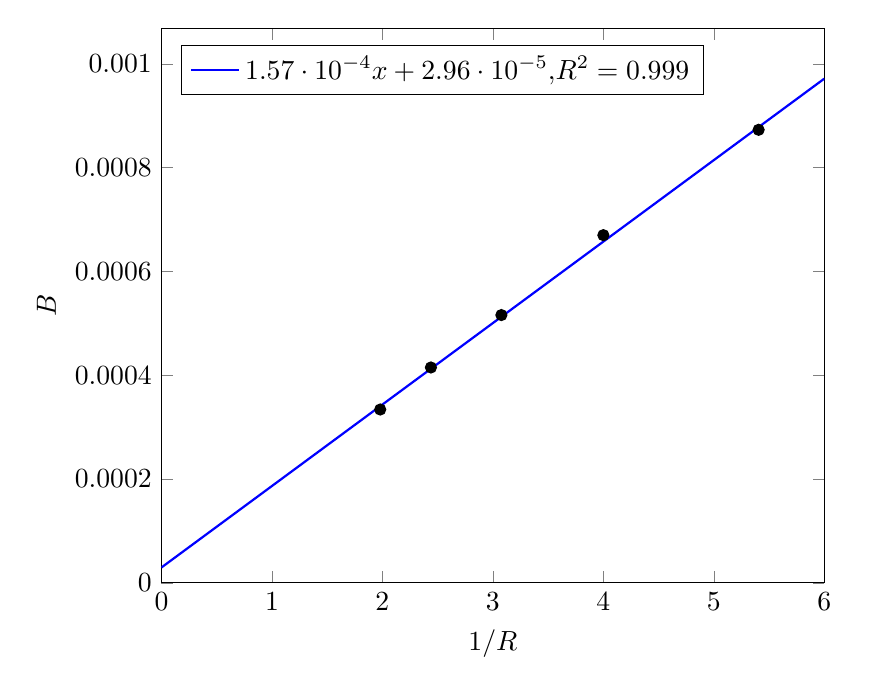
\begin{tikzpicture}
	\begin{axis}[
		xmin=0,ymin=0,
		xmax=6,
		xlabel = $1 / R$,
		ylabel = $B$,
		yticklabel style={
        		/pgf/number format/fixed,
        		/pgf/number format/precision=5
		},
		scaled y ticks = false,
		legend pos = north west
		]
		\addplot[only marks] coordinates {(1.98019802,0.000334)(2.43902439,0.000415)(3.076923077,0.000516)(4,0.000670)(5.405405405,0.000873)};
		\addplot[thick, blue, domain=0:6] {(0.000157 * x) + 0.0000296};
		\legend{,$1.57\cdot10^{-4}x+2.96\cdot 10^{-5}\text{, }R^2=0.999$}
	\end{axis}
\end{tikzpicture}\\
Figure 2: Plot of $1 / R$ vs $B$\label{fig:2}
\end{center}
\subsection{Error Analysis}\label{sec:3.3}
The error in our measurement of $e /m_e$, denoted $\Delta e/m_e$, can be given by
\[
	\Delta \frac{e}{m_e}=\sqrt{\left( \frac{2\Delta V}{B^2} \right) ^2+\left( \frac{2V\Delta B}{B^3} \right) } \cdot \frac{1}{R^2}
,\]
where $\Delta V$ and $\Delta B$ are the errors in $V$ and $B$, respectively. We know $\Delta V=1$, and we can find $\Delta B$ using
\[
	\Delta B=4.23\cdot 10^{-3}\Delta I
.\]
We know $\Delta I=0.0005$. We then have
\[
	\Delta \frac{e}{m_e}=\sqrt{\left( \frac{2}{B^2} \right) ^2+\left( \frac{2\cdot 4.23\cdot 10^{-3}\cdot 0.0005V}{B^3} \right) } \cdot R^{-2}
.\]
Since there are different $V$ and $B$ values, we will evaluate an error for each trial and take the average of the errors to be our value. Table \hyperref[tab:5]{5} depicts the error values for experiments 1 and 2.
\begin{center}
	Table 3: Errors for All Measurements\label{tab:5}\vspace{5pt}\\
	\begin{tabular}{rr}
		\toprule
		Experiment 1 Error&Experiment 2 Error\\
		\midrule
		101085535&70299872\\
		87948334&69082234\\
		78222814&71115493\\
		70241590&71285439\\
		64171804&76675859\\
		\bottomrule
	\end{tabular}
\end{center}
These numbers seem very large, but this is due to the fact that $e /m_e$ is itself very large. The average of the errors in experiment 1 is $8.033\cdot 10^{7}$, and the average in experiment 2 is $1.52\cdot 10^{8}$.

Recall that $e / m_e$ has an accepted value of $1.7588\cdot 10^{11}$, and we found values of $2.03\cdot 10^{11}$ and $2.15\cdot 10^{11}$. The absolute difference of our findings with the accepted value are
\[
	\left| 2.03-1.7588 \right| \cdot 10^{11}=2.712\cdot 10^{10}
\]
and
\[
	\left| 2.15-1.7588 \right| \cdot 10^{11}=3.912\cdot 10^{10}
\]
Since both of these values are multiple orders of magnitude above any of our errors, the data is not in agreement.
\subsection{Analysis Questions}
The report asks us to respond to the following questions.

\noindent\textbf{Question.} Does reversing the current and averaging the values compensate for the effects of Earth's Magnetic Field?

Since Earth's magnetic field is constant, the force $\mathbf{F}_E$ it exerts will always go in one direction. For example, if it's going down, then figure \ref{fig:3} shows that the total force when $\mathbf{F}_B$ is going down will be $F_B+F_E$, and otherwise it will be $F_B-F_E$. Averaging these, we find
\[
	\frac{F_B+F_E+F_B-F_E}{2}=\frac{2F_B}{2}=F_B
.\]
\begin{figure}[ht]
	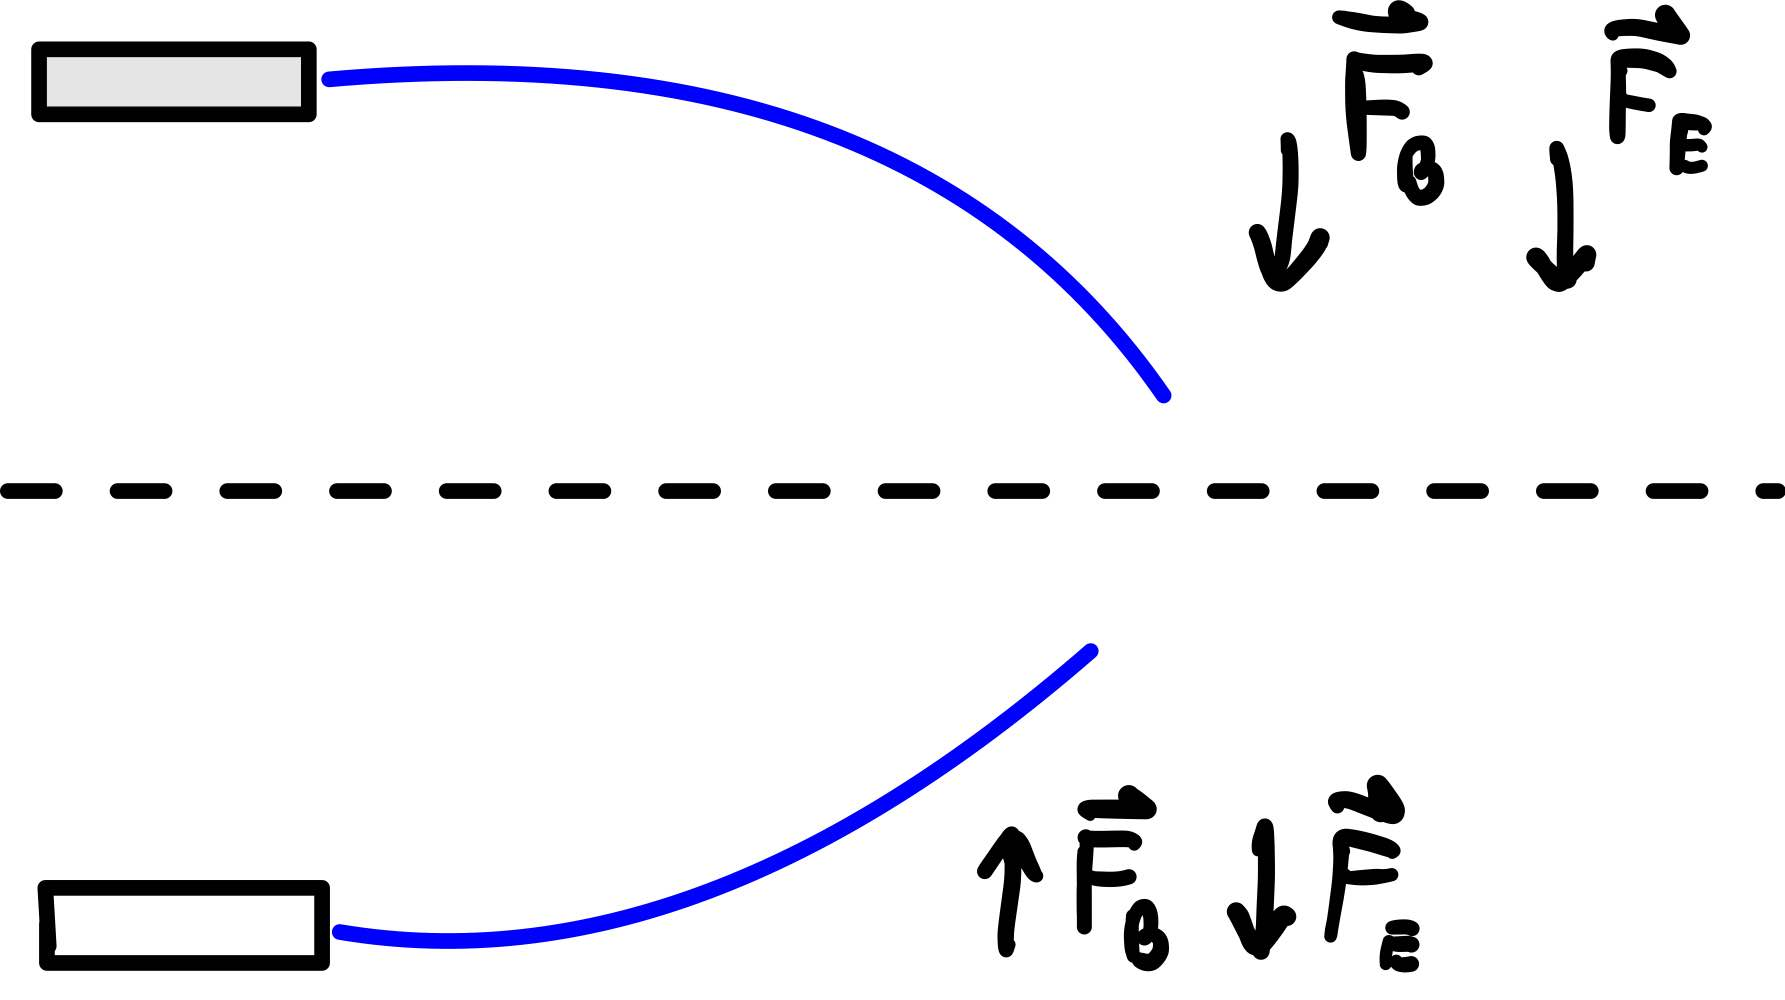
\includegraphics[scale=0.1]{diawa.jpg}
	\centering
	\setcounter{figure}{2}
	\caption{Earth's Magnetic Field}\label{fig:3}
	\centering
\end{figure}

\noindent\textbf{Question.} What is the functional dependence of the curve $B$ vs $1 /R$, depicted in figure \hyperref[fig:2]{2}? What does it represent?

Figure \hyperref[fig:2]{2} was obviously a linear relation, and excel gave the trendline $1.57\cdot 10^{-4}x+2.96\cdot 10^{-5}$. However, the reason for this relation being linear follows from equation \ref{eq:10}:
\[
	\frac{e}{m_e}=\frac{2V}{B^2R^2}
.\]
Rearranging this equation, we have
\begin{align*}
	&\qquad\;\;\;B^2=\frac{2Vm_e}{eR^2}\\
	&\implies B=\sqrt{\frac{2Vm_e}{eR^2}}=\frac{1}{R}\sqrt{\frac{2Vm_e}{e}} \\
	&\implies B\propto R^{-1}
.\end{align*}
Since we held $V$ fixed during this experiment, and since $m_e$ and $e$ are constants, we realize that the term $\sqrt{2Vm_ee^{-1}} $ is actually constant with respect to $R$, and thus the rearranged equation is linear in $R^{-1}$.

\noindent\textbf{Question.} Is the electron's velocity relativistic for the maximum considered potential?

We can use equation \ref{eq:7} to calculate this fairly simply. The maximum $V$ we considered was $V=3.2$. We will use the accepted value $e /m_e=1.7588\cdot 10^{11}$ in this calculation. We have
\begin{align*}
	v&=\sqrt{\frac{2eV}{m_e}} \\
	 &=\sqrt{2\cdot 3200\cdot 1.7588\cdot 10^{11}} \\
	 &=3355439\\
	 &=3.355439\cdot 10^{6}
.\end{align*}
Relativistic speeds are around $10^8$, and our electrons were clearly moving slower than this, as $10^6<10^8$. Therefore, the electrons did not attain relativistic speeds during our experiment.

\noindent\textbf{Question.} How would you arrange the Helmholtz coils and CRT to make the electron undergo helical motion?

The electron only undergoes circular motion if the angle between $\mathbf{B}$ and $\mathbf{v}$ is always $90^{\circ }$. If it is not $90^{\circ }$, then there will be helical motion. Thus, we simply need to offset the CRT from its current alignment perpendicular to the axis through the Helmholtz coils. Figure \ref{fig:4} depicts an aerial view of this setup, along with the directions of $\mathbf{B}$ and $\mathbf{F}$ for the initial $\mathbf{v}$.
\begin{figure}[ht]
	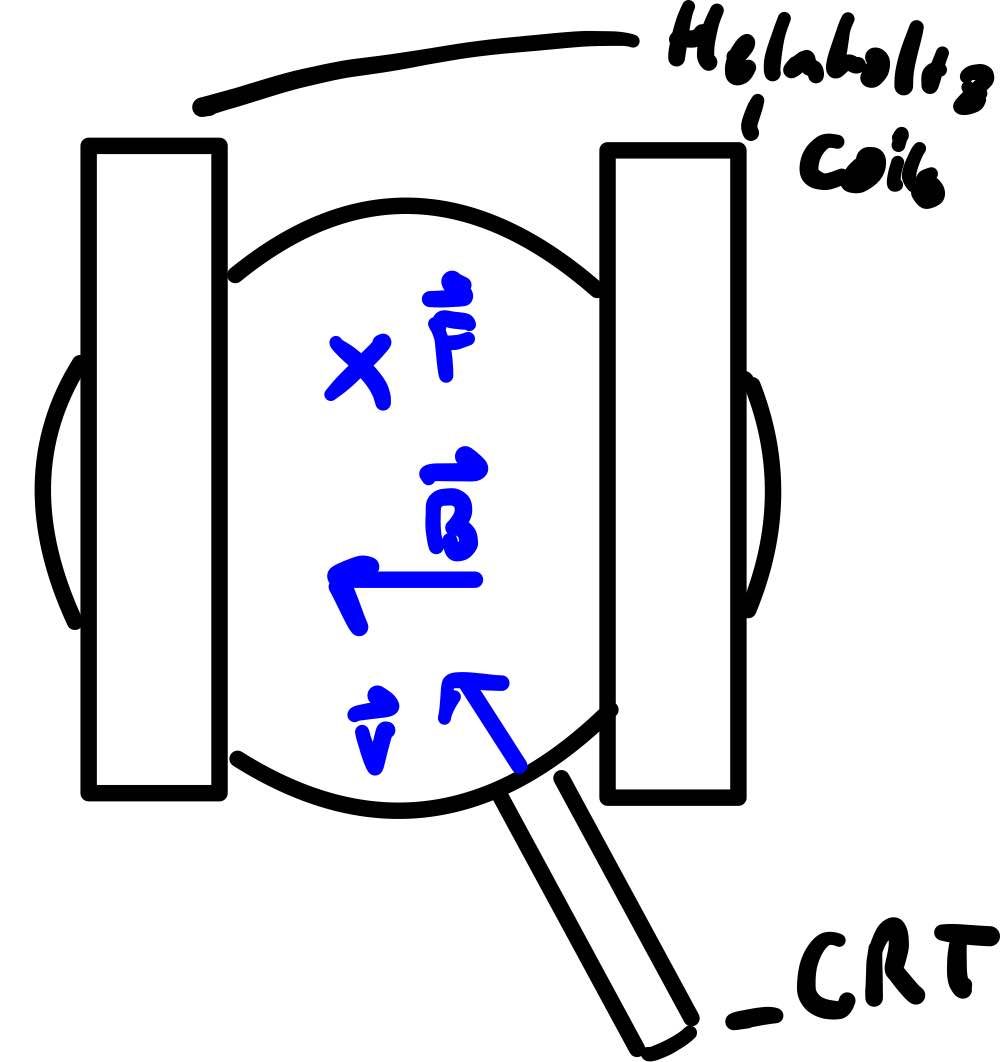
\includegraphics[scale=0.2]{diagram.jpg}
	\centering
	\caption{Modified Experimental Apparatus}\label{fig:4}
	\centering
\end{figure}
\section{Discussion}
In section \ref{sec:3.3}, we found the experimentally derived values $e /m_e $ to \emph{not} be in agreement with the accepted value, which is approximately $1.7588$ C/kg. Given that result was derived and published in a peer reviewed paper and our values are the result of 3 hours of work, it's likely that there was significant error with our measurements. We dedicate the rest of the paper to discussing these sources of error.

One highly probable source of error is the experimental apparatus itself. This author recalls touching one of the Helmholtz coils on accident and noticing a notable shift in position, so it is possible they were misaligned for a significant portion of the experiment. This would likely decrease the strength of $B$, since it would no longer be at a right angle with $\mathbf{v}$, and since equation \ref{eq:10} shows that $e / m_e\propto R^{-2}$, this would cause us to measure a value that was too large, as seen here.

Additionally, there was some error made in determining the values of $x$ and $y$ that was not accounted for. The current supplied to the Helmholtz coils was not 100\% stable, and especially for large values it would alternate within a few decimal points, and we would have to guess which value was the most precise. Furthermore, the beam was about $1 $mm in width, and as such there was extremely small error induced by the beam not necessarily being perfectly centered about each point when we measured. This error is difficult to quantify, but it was likely very small.
\end{document}
